\section{Aim of the Study}\label{aim of study}

This section describes the scope and objective of this report, and gives examples for why depthmap enhancement is needed in the purpose of achieving a better biomass estimation. The future goal towards biomass estimation is also explained. There is also a section describing some of the challenges met by working with the Raytrix technology and the underwater depthmap images. In addition, the last section describes all assumptions made in connection with the task at hand.


\subsection{Scope and Objective}

The objective of this project is enhancement of underwater color depthmap images of fish captured by the Raytrix R42 camera and generated by the Raytrix software. The depthmaps are enhanced by the use of various digital image processing techniques.
\newline

The depthmap is a color map generated by the Raytrix software, where each color represents a depth. The calibration of the camera states the depth of each color, and during calibration the object bounds are set, which determines the distance to the object. Everything behind this bound is represented with color black in the depthmap.

Due to the water mediums properties, natural particles in water and unstable lightning conditions, the depthmap produced by the Raytrix software is not exact. The object lacks some color information and particles make for some irrelevant color information to be added to the image.
If the depthmap produced by the Raytrix is to be used for volume measurement of underwater objects, it needs to be enhanced. Irrelevant data must be removed and, by the use of the correct color data, "holes" of missing color data must be filled in.
Only a complete depthmap image of an object will make for an accurate volume measurement.

The task is aimed towards fish, especially salmon, as this system would mostly benefit the salmon breeding industry. The Norwegian salmon breeding industry is currently selling their salmon in biomass, before actually knowing the total volume in each fish farm. If the fish farm is emptied and the company find that they are lacking fish, the company needs to purchase extra fish from competitors at a steep price. 
If the plenoptic camera system is able to make decent underwater volume measurements of fish, the system can be placed in every fish farm and be used to estimate the total volume in each farm, and this will profit the companies directly.

A depthmap computed by the Raytrix camera under good conditions normally looks like the one in figure \ref{fig:depthmap82}. It is seen from this image that there are large "holes" in the fish, color information for much of the head and belly is missing, and all red pixels represent particles in front of the fish. The depthmap has potential for both simple and advanced improvement, but there are also some challenges working with the Raytrix technology.

\begin{figure}[H]
    \centering
    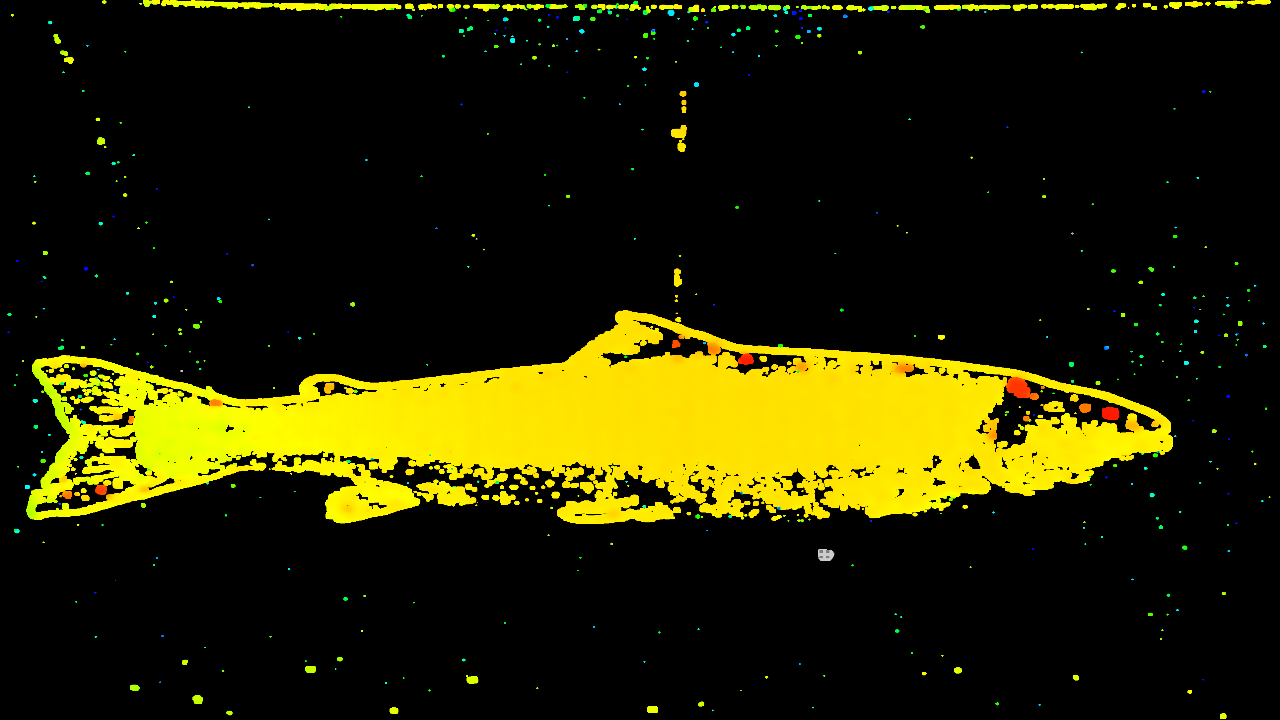
\includegraphics[width=.7\linewidth]{images/aim_of_study/depthmap82}
    \caption{Depthmap image of salmon}
    \label{fig:depthmap82}
\end{figure}



\subsubsection{Challenges}

A MATLAB 3D plot shows how insufficient the information contained in the original depthmap generated by the Raytrix is (see figure \ref{fig:matlab3D}). It is plotted by the use of color intensity for depth. The particles make for large disturbances and the holes in the fish make for even bigger ones. The parts of the salmon that make for the largest depthmap errors is the belly, the fins and its head. The belly is white and the color is too close the the background color in the test facility. The head and fins are very black, and it could be a problem to the Raytrix that it is too black over a certain area, and therefore makes it hard to see differences in each micro lens. (See section \ref{the_raytrix_camera}, for detailed information about the Raytrix camera technology.)

\begin{figure}[H]
    \centering
    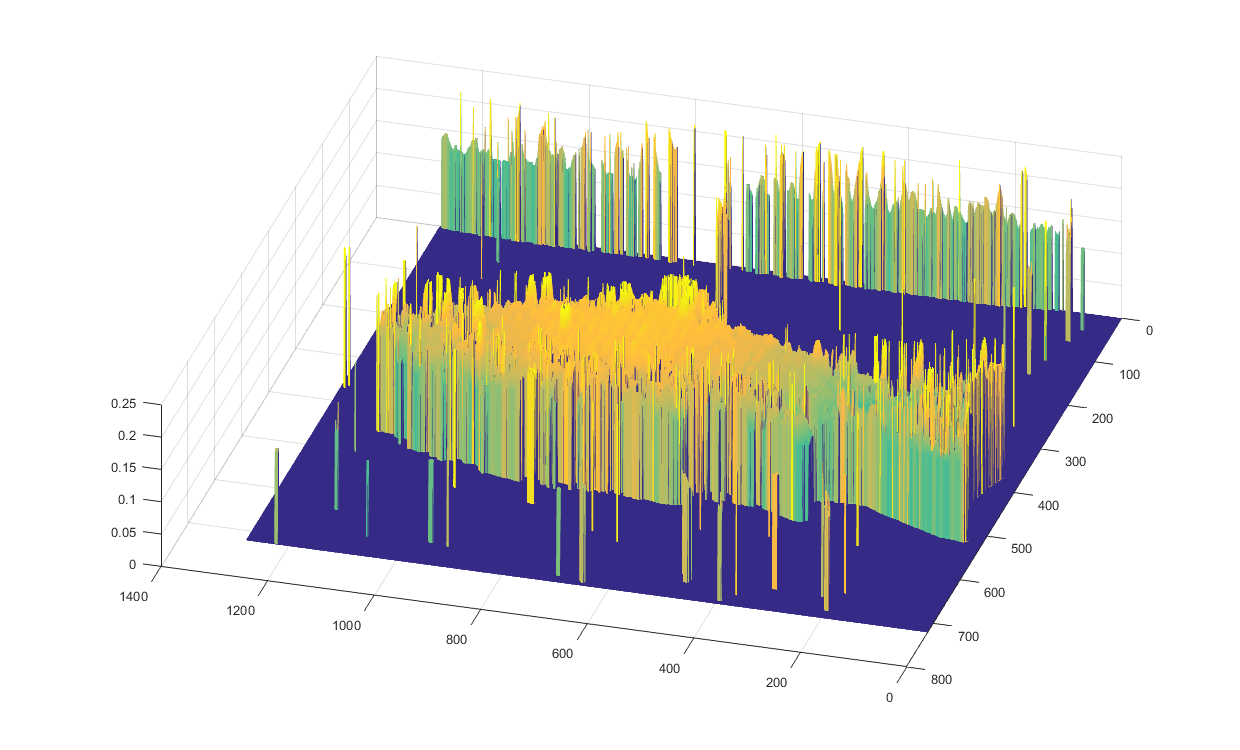
\includegraphics[width=.7\linewidth]{images/aim_of_study/original_3D_87}
    \caption{3D plot of depthmap}
    \label{fig:matlab3D}
\end{figure}

The Raytrix R42 camera has no documentation for underwater usage. Therefore, testing in different conditions is important for achieving a good base depthmap image. Raytrix also uses its own software, which has no compatibility with other image processing tools. When the depthmap image is taken out from the Raytrix software and modified it cannot be converted back to the raytrix format for further processing in the Raytrix software. As the actual depth information is not stored in the color from the depthmap alone, but in a combination of the depthmap color and the camera calibration information, also the calibration data needs to be considered when actual depth data is needed for future use. 



\subsection{Assumptions}

For this project, only modifications to the depthmap itself is made, where the goal is for the whole fish in the depthmap to be given relevant color values and for the colors in the depthmap to be smoothed out so it at the end represents a smooth surface with the correct color data from the original depthmap preserved. This assumption can be made since the main object for this task is fish, and most fish relevant for this task has a smooth surface, and no sharp or pointy edges that affects the volume. 

During image taking, dead Atlantic Salmon has been used, and the fish is therefore held still at a certain position that is set during camera calibration, and it does not move during image taking. This is for the reason that good images containing the whole fish would be hard to achieve if the fish was swimming around in the test facility.

It is also assumed that the images of fish is taken at a 90 degree angle on the fish, as in figure \ref{fig:depthmap82}, and that there is only one object in the area of interest at each time. Objects behind the area of interest set during camera calibration will not affect the outcome, while objects too close to the camera will disturb the shape of the object of interest. Therefore, the report only considers one object at a time in front of the camera.

Even though there are many challenges, it should be possible to enhance the depthmap from the Raytrix to get a smooth surface of the fish, while preserving the shape and the correct color data. That is what the following sections in this report hope to show using the theory provided in section \ref{theory}.